% chapters/ch03.tex
\chapter{Marco metodológico}

\begin{refsection}
\addbibresource{references/ch03.bib}
\section{Arquitectura metodológica de la investigación}

Con el propósito de ofrecer una visión integrada del diseño metodológico de la investigación, se presenta una arquitectura conceptual que sintetiza la relación entre el problema educativo identificado, el marco teórico que fundamenta el estudio, el enfoque metodológico adoptado y el proceso de desarrollo y validación del sistema tecnológico propuesto.

La Figura \ref{fig:arquitectura-metodologica} representa la estructura metodológica general del estudio, integrando el enfoque de métodos mixtos, el diseño de Investigación Basada en el Diseño (Design-Based Research -- DBR) y el proceso de desarrollo del sistema tecnológico de diagnóstico educativo inclusivo.

\begin{figure}[htbp]
\centering
\resizebox{\textwidth}{!}{%
\begin{tikzpicture}[
font=\footnotesize,
node distance=12mm,
box/.style={draw, rounded corners=2mm, align=center, inner sep=7pt, text width=4.5cm},
big/.style={draw, rounded corners=2mm, align=center, inner sep=9pt, text width=7cm},
arrow/.style={-{Stealth[length=2.5mm]}, thick}
]

% Problema
\node[big] (problem)
{\textbf{Problema de investigación}\\
Diagnósticos educativos insuficientes para comprender la diversidad del aprendizaje};

% Preguntas
\node[big, below=of problem] (questions)
{\textbf{Preguntas de investigación}\\
Diseño, implementación y validación de un sistema tecnológico inteligente de diagnóstico educativo inclusivo};

% Marco teórico
\node[big, below=of questions] (theory)
{\textbf{Marco teórico}\\
Inclusión educativa\\
Diseño Universal para el Aprendizaje\\
Educación basada en datos};

% Enfoque metodológico
\node[big, below=of theory] (method)
{\textbf{Enfoque metodológico}\\
Métodos mixtos\\
Paradigma pragmático};

% DBR
\node[big, below=of method] (dbr)
{\textbf{Diseño metodológico}\\
Investigación Basada en el Diseño (DBR)};

% Desarrollo del sistema
\node[box, below left=of dbr] (design)
{Diseño del sistema tecnológico};

\node[box, below=of dbr] (implementation)
{Implementación en contexto educativo};

\node[box, below right=of dbr] (evaluation)
{Evaluación y análisis de resultados};

% Contribuciones
\node[big, below=22mm of dbr] (contributions)
{\textbf{Aportes científicos}\\
Modelo de diagnóstico educativo inclusivo basado en datos\\
Sistema tecnológico inteligente\\
Conocimiento transferible};

% Flechas
\draw[arrow] (problem) -- (questions);
\draw[arrow] (questions) -- (theory);
\draw[arrow] (theory) -- (method);
\draw[arrow] (method) -- (dbr);

\draw[arrow] (dbr) -- (design);
\draw[arrow] (dbr) -- (implementation);
\draw[arrow] (dbr) -- (evaluation);

\draw[arrow] (design) -- (contributions);
\draw[arrow] (implementation) -- (contributions);
\draw[arrow] (evaluation) -- (contributions);

\end{tikzpicture}
}
\caption{Arquitectura metodológica de la investigación doctoral.}
\label{fig:arquitectura-metodologica}
\end{figure}

Como se observa en la Figura \ref{fig:arquitectura-metodologica}, la investigación se estructura a partir de la identificación de un problema educativo relacionado con las limitaciones de los diagnósticos educativos tradicionales para comprender la diversidad del aprendizaje.

A partir de este problema se formulan preguntas de investigación que orientan el desarrollo del estudio y que se sustentan en un marco teórico que integra los enfoques de inclusión educativa, Diseño Universal para el Aprendizaje y educación basada en datos.

Sobre esta base conceptual se adopta un enfoque metodológico de métodos mixtos dentro de un paradigma pragmático, el cual permite integrar análisis cuantitativos y cualitativos en el estudio del fenómeno educativo.

El diseño metodológico se fundamenta en la Investigación Basada en el Diseño (DBR), que permite desarrollar, implementar y refinar iterativamente el sistema tecnológico propuesto en contextos educativos reales. Este proceso conduce finalmente a la generación de aportes científicos orientados tanto al desarrollo de un modelo conceptual de diagnóstico educativo inclusivo basado en datos como a la construcción de un sistema tecnológico capaz de apoyar la toma de decisiones pedagógicas en contextos educativos diversos.
\section{Enfoque de la investigación}

La presente investigación se desarrolla bajo un \textbf{enfoque mixto}, integrando métodos cuantitativos y cualitativos con el propósito de abordar de manera integral la complejidad del \textbf{diagnóstico educativo inclusivo mediado por tecnología}. En coherencia con la naturaleza del problema y con el objetivo de diseñar, implementar y validar un sistema tecnológico inteligente, el enfoque mixto permite articular:

\begin{itemize}
\item \textbf{un componente cuantitativo} orientado al análisis de datos educativos, la identificación de patrones de aprendizaje, la construcción de indicadores y la evaluación empírica del desempeño del sistema y de sus diagnósticos;
\item \textbf{un componente cualitativo} orientado a comprender las percepciones, experiencias, valoraciones y condiciones de uso del sistema por parte de los actores educativos (docentes, estudiantes y directivos cuando aplique), así como los factores contextuales que inciden en la pertinencia y accesibilidad de la intervención.
\end{itemize}

De acuerdo con \textcite{creswell2018}, los métodos mixtos resultan especialmente pertinentes en investigaciones educativas que diseñan y evalúan intervenciones complejas, dado que permiten integrar resultados observables con interpretaciones contextualizadas, fortaleciendo la validez del estudio.

\section{Paradigma y diseño metodológico}

\subsection{Paradigma de investigación}

La investigación se inscribe en un \textbf{paradigma pragmático}, el cual prioriza la utilidad del conocimiento generado para la resolución de problemas educativos concretos y reconoce que diferentes estrategias metodológicas pueden ser necesarias para comprender fenómenos educativos multidimensionales.

Desde este paradigma, el valor del conocimiento no se reduce a su coherencia teórica, sino que se vincula a su capacidad para orientar decisiones educativas, mejorar prácticas pedagógicas y producir resultados aplicables en contextos reales. El paradigma pragmático posibilita:

\begin{itemize}
\item combinar métodos y técnicas de investigación de manera coherente;
\item orientar la producción de conocimiento hacia la \textbf{mejora educativa} y la reducción de barreras;
\item articular teoría, práctica, ética y tecnología en un mismo marco interpretativo.
\end{itemize}

Este enfoque resulta consistente con discusiones contemporáneas sobre educación, medición y responsabilidad ética en contextos de toma de decisiones basadas en evidencia \parencite{biesta2010}.

\subsection{Diseño metodológico: Design-Based Research (DBR)}

El diseño metodológico adoptado corresponde a la \textbf{Investigación Basada en el Diseño} (\DBR). Este enfoque es adecuado cuando el objetivo de la investigación implica diseñar y mejorar una intervención educativa en contextos reales, produciendo simultáneamente aportes prácticos y conocimiento científico transferible.

De acuerdo con \textcite{wang2005}, la \DBR\ se caracteriza por:

\begin{itemize}
\item el diseño y desarrollo de una intervención educativa (en esta investigación, un sistema tecnológico inteligente);
\item la implementación en contextos auténticos de enseñanza y aprendizaje;
\item la evaluación sistemática de procesos y resultados;
\item el refinamiento iterativo a partir de evidencia empírica y retroalimentación de los actores educativos.
\end{itemize}

En esta investigación, la lógica iterativa de la \DBR\ permite ajustar progresivamente: (i) los instrumentos digitales de captura de datos, (ii) los indicadores e inferencias diagnósticas, (iii) los criterios de accesibilidad y usabilidad, y (iv) la interpretabilidad pedagógica de los reportes y recomendaciones.

La Figura \ref{fig:dbr-ciclo} sintetiza el ciclo iterativo aplicado.

\begin{figure}[htbp]
\centering
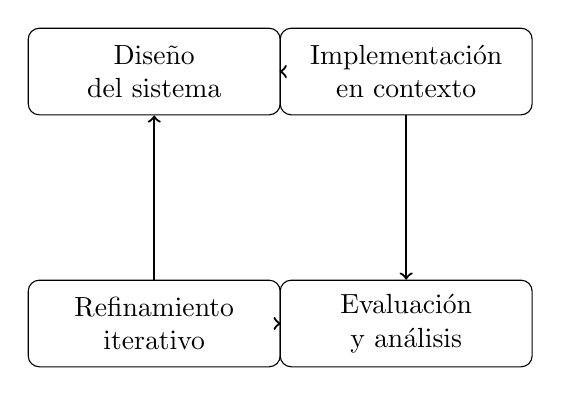
\begin{tikzpicture}[
node distance=3.2cm,
every node/.style={draw, rounded corners, align=center, minimum width=3.2cm, minimum height=1.1cm},
arrow/.style={->, thick}
]
\node (design) {Diseño\\del sistema};
\node (implementation) [right of=design] {Implementación\\en contexto};
\node (evaluation) [below of=implementation] {Evaluación\\y análisis};
\node (refinement) [left of=evaluation] {Refinamiento\\iterativo};

\draw[arrow] (design) -- (implementation);
\draw[arrow] (implementation) -- (evaluation);
\draw[arrow] (evaluation) -- (refinement);
\draw[arrow] (refinement) -- (design);
\end{tikzpicture}
\caption{Ciclo iterativo de \DBR\ aplicado al desarrollo del sistema tecnológico de diagnóstico educativo inclusivo.}
\label{fig:dbr-ciclo}
\end{figure}

\section{Contexto y participantes}

La investigación se desarrolla en un \textbf{contexto educativo real}, seleccionado bajo criterios de pertinencia, accesibilidad, viabilidad y diversidad educativa, con el fin de observar el funcionamiento del sistema en situaciones auténticas.

Los participantes incluyen:

\begin{itemize}
\item \textbf{docentes}, quienes interactúan con reportes, paneles y recomendaciones pedagógicas;
\item \textbf{estudiantes}, quienes aportan datos a través de instrumentos y registros de interacción (según corresponda al diseño del sistema);
\item \textbf{actores institucionales} (directivos u orientadores), cuando el contexto lo requiera para comprender políticas, rutas de atención o decisiones institucionales.
\end{itemize}

La selección se realiza mediante \textbf{muestreo intencional}, priorizando la diversidad de perfiles, trayectorias educativas y condiciones contextuales, con el fin de fortalecer la pertinencia inclusiva del análisis. Dado el carácter aplicado y contextual del estudio, los resultados se orientan a la \textbf{transferibilidad} conceptual y metodológica hacia contextos similares, más que a la generalización estadística.

\section{Instrumentos de recolección de información}

\subsection{Sistema tecnológico inteligente como instrumento principal}

El instrumento central de la investigación es el \textbf{sistema tecnológico inteligente} desarrollado, concebido simultáneamente como:

\begin{itemize}
\item \textbf{intervención educativa} orientada al diagnóstico inclusivo basado en datos;
\item \textbf{instrumento científico} para la recolección, organización y análisis de información educativa.
\end{itemize}

En términos operativos, el sistema permite:

\begin{itemize}
\item capturar información mediante instrumentos digitales y registros de interacción;
\item estructurar y almacenar datos educativos de manera sistemática;
\item aplicar analítica del aprendizaje y reglas/criterios de diagnóstico inclusivo;
\item generar reportes interpretables y recomendaciones pedagógicas alineadas con el \DUA;
\item asegurar trazabilidad del proceso diagnóstico (evidencias, variables e inferencias).
\end{itemize}

La Figura \ref{fig:arquitectura-sistema} presenta una arquitectura funcional de alto nivel.

\begin{figure}[htbp]
\centering
\resizebox{\textwidth}{!}{%
\begin{tikzpicture}[
font=\footnotesize,
node distance=10mm,
layer/.style={draw, rounded corners=2mm, align=center, inner sep=8pt, text width=10cm},
arrow/.style={->, thick}
]
\node[layer] (users) {Actores educativos\\Docentes — Estudiantes — Instituciones};

\node[layer, below=of users] (ui)
{Capa de interacción\\Plataforma digital de diagnóstico educativo};

\node[layer, below=of ui] (ped)
{Capa pedagógica\\Recomendaciones didácticas alineadas con \DUA};

\node[layer, below=of ped] (diagnosis)
{Motor de diagnóstico educativo inclusivo\\(perfiles, barreras, apoyos, evidencias)};

\node[layer, below=of diagnosis] (analytics)
{Capa de analítica del aprendizaje\\(indicadores, patrones, métricas e inferencias)};

\node[layer, below=of analytics] (data)
{Capa de datos educativos\\(instrumentos, registros, contexto, resguardos éticos)};

\draw[arrow] (users) -- (ui);
\draw[arrow] (ui) -- (ped);
\draw[arrow] (ped) -- (diagnosis);
\draw[arrow] (diagnosis) -- (analytics);
\draw[arrow] (analytics) -- (data);
\end{tikzpicture}
}
\caption{Arquitectura funcional del sistema tecnológico de diagnóstico educativo inclusivo basado en datos.}
\label{fig:arquitectura-sistema}
\end{figure}
\section{Arquitectura del sistema tecnológico}

Con el fin de representar de manera integral la estructura técnica del sistema propuesto, se presenta la arquitectura general del sistema tecnológico de diagnóstico educativo inclusivo basado en datos. Esta arquitectura articula componentes de interacción, procesamiento, analítica del aprendizaje, inteligencia artificial, almacenamiento de datos y criterios transversales de accesibilidad y ética.

La Figura \ref{fig:arquitectura-completa-sistema} sintetiza los principales módulos del sistema y sus relaciones funcionales.

\begin{figure}[htbp]
\centering
\resizebox{\textwidth}{!}{%
\begin{tikzpicture}[
font=\footnotesize,
node distance=10mm and 12mm,
box/.style={draw, rounded corners=2mm, align=center, inner sep=6pt, text width=4.1cm},
bigbox/.style={draw, rounded corners=2mm, align=center, inner sep=8pt, text width=8.2cm},
layer/.style={draw, rounded corners=2mm, align=center, inner sep=8pt, text width=12.5cm},
arrow/.style={-{Stealth[length=2.6mm]}, thick, rounded corners=2pt}
]

%------------------------------------------------
% Actores
%------------------------------------------------
\node[box] (docentes) {Docentes\\Consulta de reportes\\y toma de decisiones};
\node[box, right=of docentes] (estudiantes) {Estudiantes\\Interacción con actividades\\e instrumentos};
\node[box, right=of estudiantes] (instituciones) {Instituciones\\Seguimiento, apoyo\\y gestión educativa};

%------------------------------------------------
% Frontend
%------------------------------------------------
\node[layer, below=of estudiantes] (frontend)
{\textbf{Capa de interacción / Frontend}\\
Aplicación web + aplicación móvil\\
Interfaces accesibles, formularios, paneles, visualización de resultados};

\draw[arrow] (docentes) -- (frontend);
\draw[arrow] (estudiantes) -- (frontend);
\draw[arrow] (instituciones) -- (frontend);

%------------------------------------------------
% Backend
%------------------------------------------------
\node[layer, below=of frontend] (backend)
{\textbf{Capa de servicios / Backend}\\
Gestión de usuarios \quad $\cdot$ \quad autenticación \quad $\cdot$ \quad APIs\\
orquestación de procesos \quad $\cdot$ \quad reglas del sistema};

\draw[arrow] (frontend) -- (backend);

%------------------------------------------------
% Módulos internos
%------------------------------------------------
\node[box, below left=12mm and 18mm of backend] (capture)
{Módulo de captura\\de datos educativos\\(cuestionarios, registros, contexto)};

\node[box, below=12mm of backend] (analytics)
{Motor de analítica\\del aprendizaje\\(indicadores, patrones, perfiles)};

\node[box, below right=12mm and 18mm of backend] (ai)
{Módulo de IA\\e inferencia diagnóstica\\(reglas, clasificación, apoyo)};

\draw[arrow] (backend) -- (capture);
\draw[arrow] (backend) -- (analytics);
\draw[arrow] (backend) -- (ai);

%------------------------------------------------
% Base de datos
%------------------------------------------------
\node[bigbox, below=14mm of analytics] (database)
{\textbf{Base de datos educativa}\\
Datos pedagógicos \quad $\cdot$ \quad datos contextuales \quad $\cdot$ \quad registros de interacción\\
perfiles de usuario \quad $\cdot$ \quad resultados diagnósticos \quad $\cdot$ \quad bitácoras de uso};

\draw[arrow] (capture) -- (database);
\draw[arrow] (analytics) -- (database);
\draw[arrow] (ai) -- (database);

\draw[arrow] (database.north) -- ($(database.north)+(0,5mm)$) -| (analytics.south);
\draw[arrow] (database.north) -- ($(database.north)+(0,5mm)$) -| (ai.south);

%------------------------------------------------
% Salidas
%------------------------------------------------
\node[box, below left=14mm and 10mm of database] (reports)
{Reportes diagnósticos\\interpretables\\para docentes};

\node[box, below=14mm of database] (recommend)
{Recomendaciones pedagógicas\\alineadas con DUA};

\node[box, below right=14mm and 10mm of database] (monitoring)
{Monitoreo y mejora\\continua del sistema};

\draw[arrow] (database) -- (reports);
\draw[arrow] (database) -- (recommend);
\draw[arrow] (database) -- (monitoring);

%------------------------------------------------
% Retroalimentación
%------------------------------------------------
\draw[arrow] (reports.north) -- ($(reports.north)+(0,7mm)$) -| (frontend.south);
\draw[arrow] (recommend.north) -- ($(recommend.north)+(0,7mm)$) -| (frontend.south);
\draw[arrow] (monitoring.north) -- ($(monitoring.north)+(0,7mm)$) -| (backend.south);

%------------------------------------------------
% Criterios transversales
%------------------------------------------------
\node[bigbox, below=18mm of recommend] (ethics)
{\textbf{Criterios transversales de accesibilidad y ética}\\
Accesibilidad digital \quad $\cdot$ \quad usabilidad \quad $\cdot$ \quad privacidad \quad $\cdot$ \quad protección de datos\\
transparencia \quad $\cdot$ \quad no discriminación algorítmica \quad $\cdot$ \quad seguridad};

\draw[arrow] (ethics.north) -- ($(ethics.north)+(0,7mm)$) -| (reports.south);
\draw[arrow] (ethics.north) -- ($(ethics.north)+(0,7mm)$) -| (recommend.south);
\draw[arrow] (ethics.north) -- ($(ethics.north)+(0,7mm)$) -| (monitoring.south);

\end{tikzpicture}
}
\caption{Arquitectura completa del sistema tecnológico de diagnóstico educativo inclusivo basado en datos.}
\label{fig:arquitectura-completa-sistema}
\end{figure}

Como se observa en la Figura \ref{fig:arquitectura-completa-sistema}, el sistema se organiza en múltiples capas funcionales. En la parte superior se encuentran los actores educativos que interactúan con la plataforma mediante interfaces web y móviles. A continuación, una capa de servicios coordina autenticación, gestión de usuarios y orquestación de procesos.

En el núcleo del sistema se sitúan tres módulos principales: el módulo de captura de datos educativos, el motor de analítica del aprendizaje y el módulo de inteligencia artificial e inferencia diagnóstica. Estos componentes interactúan con una base de datos educativa en la cual se almacenan evidencias de aprendizaje, variables contextuales, perfiles de usuario y resultados diagnósticos.

A partir de este procesamiento, el sistema genera reportes interpretables, recomendaciones pedagógicas alineadas con el \DUA\ y mecanismos de monitoreo orientados a la mejora continua. Finalmente, la arquitectura incorpora criterios transversales de accesibilidad y ética, que garantizan que el funcionamiento del sistema se mantenga alineado con principios de inclusión, privacidad, transparencia y no discriminación.


\section{Trazabilidad funcional del sistema tecnológico}

Con el propósito de garantizar la coherencia entre la arquitectura tecnológica del sistema y los principios pedagógicos y éticos que orientan la investigación, se presenta una matriz de trazabilidad funcional. Esta matriz relaciona los módulos principales del sistema con sus funciones, las entradas de información que procesan, las salidas que generan y los criterios de accesibilidad y ética incorporados en su diseño.

La Tabla \ref{tab:trazabilidad-sistema} sintetiza esta relación.

\begin{APAlongtable}
{@{}p{3cm}p{3.5cm}p{3cm}p{3cm}p{2.8cm}p{2.5cm}@{}}
{Matriz de trazabilidad funcional del sistema tecnológico de diagnóstico educativo inclusivo.}
{tab:trazabilidad-sistema}

\textbf{Módulo del sistema} &
\textbf{Función principal} &
\textbf{Entradas} &
\textbf{Salidas} &
\textbf{Criterios de accesibilidad} &
\textbf{Criterios éticos} \\
\midrule
\endfirsthead

\toprule
\textbf{Módulo del sistema} &
\textbf{Función principal} &
\textbf{Entradas} &
\textbf{Salidas} &
\textbf{Criterios de accesibilidad} &
\textbf{Criterios éticos} \\
\midrule
\endhead

\midrule
\multicolumn{6}{r}{\APAtablecontinued}\\
\endfoot

\endlastfoot

Captura de datos educativos &
Recopilar información pedagógica y contextual del estudiante &
Respuestas a cuestionarios, registros de interacción, datos contextuales &
Base de datos educativa estructurada &
Interfaces accesibles, formularios claros, navegación simple &
Consentimiento informado, minimización de datos \\

Gestión de usuarios &
Administrar cuentas, roles y permisos de acceso &
Datos de registro de usuarios, credenciales de autenticación &
Perfiles de usuario y control de acceso &
Interfaces comprensibles y navegación accesible &
Protección de identidad y seguridad de credenciales \\

Motor de analítica del aprendizaje &
Procesar datos educativos para identificar patrones de aprendizaje &
Datos pedagógicos, registros de interacción, variables contextuales &
Indicadores de aprendizaje y perfiles educativos &
Visualización clara de resultados analíticos &
Prevención de sesgos analíticos \\

Módulo de inferencia diagnóstica &
Generar diagnósticos educativos inclusivos basados en evidencia &
Indicadores analíticos, variables educativas, perfiles de aprendizaje &
Diagnóstico educativo contextualizado &
Presentación comprensible del diagnóstico &
Transparencia en criterios diagnósticos \\

Generación de recomendaciones pedagógicas &
Proponer estrategias didácticas alineadas con el \DUA &
Resultados diagnósticos y perfiles de aprendizaje &
Recomendaciones pedagógicas diferenciadas &
Adaptación de contenidos a diversos usuarios &
Evitar etiquetado o estigmatización \\

Panel docente de visualización &
Presentar información diagnóstica para apoyar la toma de decisiones pedagógicas &
Resultados analíticos y diagnósticos generados &
Reportes pedagógicos y visualizaciones de datos &
Visualización accesible y clara de la información &
Uso responsable de datos educativos \\

Sistema de monitoreo y mejora &
Registrar el funcionamiento del sistema y retroalimentación del usuario &
Registros de uso, retroalimentación docente, métricas del sistema &
Mejoras iterativas del sistema tecnológico &
Interfaz simple para reportar incidencias &
Auditoría de procesos y transparencia \\

Base de datos educativa &
Almacenar de manera estructurada los datos educativos y resultados diagnósticos &
Datos capturados, indicadores analíticos, diagnósticos generados &
Repositorio estructurado de datos educativos &
Acceso estructurado a la información &
Anonimización y protección de datos \\

\end{APAlongtable}
\subsection{Cuestionarios e instrumentos diagnósticos complementarios}

Se emplean cuestionarios estructurados y semiestructurados para:

\begin{itemize}
\item caracterizar variables pedagógicas, cognitivas, contextuales y socioeducativas relevantes;
\item levantar información sobre percepciones de accesibilidad, usabilidad y utilidad pedagógica;
\item complementar la evidencia capturada por registros de interacción del sistema.
\end{itemize}

Los instrumentos se someten a \textbf{validación de contenido} mediante juicio de expertos y, cuando corresponda, análisis de consistencia interna, siguiendo recomendaciones metodológicas ampliamente utilizadas en investigación educativa \parencite{hernandez2014}.

\subsection{Técnicas cualitativas}

Como complemento, se utilizan técnicas cualitativas orientadas a comprender el sentido pedagógico del diagnóstico y las condiciones reales de implementación:

\begin{itemize}
\item entrevistas semiestructuradas a docentes (y a actores institucionales cuando aplique);
\item análisis de documentos institucionales (PEI, lineamientos, rutas, planes de apoyo);
\item observación del uso del sistema (sesiones, acompañamiento, incidencias de accesibilidad).
\end{itemize}

Estas técnicas permiten contextualizar los resultados cuantitativos y fortalecer la interpretación, evitando lecturas reduccionistas de los datos.
\section{Matriz de operacionalización}

Con el fin de asegurar coherencia entre las preguntas de investigación, los constructos teóricos, las variables consideradas y las decisiones metodológicas, se presenta la matriz de operacionalización. Esta matriz establece el vínculo entre: (i) preguntas de investigación, (ii) variables/dimensiones analíticas, (iii) indicadores observables, (iv) instrumentos y fuentes de datos, y (v) técnicas de análisis. Su función es fortalecer la trazabilidad del estudio y la consistencia entre el diseño conceptual y el procedimiento empírico.

% --- Tabla multipágina con encabezado repetido ---
\begin{APAlongtable}
{@{}p{3.0cm}p{3.0cm}Y p{3.0cm}p{2.6cm}@{}}
{Matriz de operacionalización: preguntas, variables, indicadores, instrumentos y análisis.}
{tab:operacionalizacion}

\textbf{Pregunta de investigación} &
\textbf{Variable / Dimensión} &
\textbf{Indicadores observables (ejemplos)} &
\textbf{Instrumento / Fuente} &
\textbf{Técnica de análisis} \\
\midrule
\endfirsthead

\toprule
\textbf{Pregunta de investigación} &
\textbf{Variable / Dimensión} &
\textbf{Indicadores observables (ejemplos)} &
\textbf{Instrumento / Fuente} &
\textbf{Técnica de análisis} \\
\midrule
\endhead

\midrule
\multicolumn{5}{r}{\APAtablecontinued}\\
\endfoot

\endlastfoot

% =========================
% P1: Fundamentos teóricos/pedagógicos/tecnológicos/normativos
% =========================
\textbf{P1. Fundamentos que sustentan el diagnóstico inclusivo} &
Marco normativo y ético &
Presencia de principios de inclusión, equidad, accesibilidad, privacidad y no discriminación; criterios explícitos de gobernanza de datos &
Revisión documental; análisis de marcos institucionales y normativos; literatura científica &
Análisis documental; síntesis temática \\

\textbf{P1. Fundamentos que sustentan el diagnóstico inclusivo} &
Marco pedagógico (\DUA) &
Correspondencia entre principios del \DUA\ y requerimientos diagnósticos; coherencia entre diagnóstico y apoyos pedagógicos &
Revisión teórica; validación conceptual del modelo; juicio de expertos &
Análisis conceptual; validación de contenido \\

% =========================
% P2: Variables para diagnóstico inclusivo basado en datos
% =========================
\textbf{P2. Variables para construir el diagnóstico inclusivo} &
Variables pedagógicas &
Variedad de estrategias; diferenciación; participación; adecuaciones/apoyos implementados &
Rúbrica docente; observación guiada; registros del sistema &
Descriptivo; análisis de patrones; triangulación \\

\textbf{P2. Variables para construir el diagnóstico inclusivo} &
Variables cognitivas (orientativas) &
Ritmo/progresión; persistencia; uso de estrategias; patrones de interacción con recursos &
Registros del sistema; instrumentos de autorregulación; cuestionario orientativo &
Analítica del aprendizaje; descriptivo/inferencial (si aplica) \\

\textbf{P2. Variables para construir el diagnóstico inclusivo} &
Variables contextuales &
Acceso a conectividad/recursos; barreras físicas/tecnológicas; apoyos institucionales disponibles &
Encuesta contextual; checklist de accesibilidad; entrevista institucional &
Descriptivo; análisis temático; mapas de barreras \\

\textbf{P2. Variables para construir el diagnóstico inclusivo} &
Variables socioeducativas &
Motivación, autoeficacia, compromiso; interacción social; percepción de apoyo &
Cuestionarios; entrevistas; observación estructurada; registros de interacción &
Análisis temático; integración con métricas de participación \\

% =========================
% P3: Modelo conceptual del sistema (datos + accesibilidad + inclusión)
% =========================
\textbf{P3. Modelo conceptual del sistema tecnológico} &
Arquitectura funcional y trazabilidad &
Existencia de módulos; flujo datos$\rightarrow$analítica$\rightarrow$diagnóstico$\rightarrow$recomendación; auditabilidad de decisiones &
Documentación técnica; diagrama de arquitectura; bitácora de diseño (\DBR) &
Análisis de trazabilidad; revisión por expertos \\

\textbf{P3. Modelo conceptual del sistema tecnológico} &
Accesibilidad y usabilidad &
Cumplimiento de criterios de accesibilidad (interacción, navegación, lectura); facilidad de uso; barreras de interfaz identificadas &
Pruebas de usabilidad; checklist de accesibilidad; retroalimentación de usuarios &
Análisis descriptivo; análisis temático; priorización de mejoras \\

% =========================
% P4: Integración analítica del aprendizaje e IA
% =========================
\textbf{P4. Integración de analítica del aprendizaje e \IA} &
Modelos/Reglas diagnósticas &
Definición de variables de entrada; indicadores; reglas o modelos; consistencia de inferencias; explicabilidad &
Módulo analítico del sistema; bitácora; pruebas funcionales; revisión experta &
Evaluación técnica; validación de contenido; análisis de consistencia \\

\textbf{P4. Integración de analítica del aprendizaje e \IA} &
Rendimiento y estabilidad &
Tasa de error; tiempos de respuesta; completitud de datos; consistencia en ejecuciones &
Logs del sistema; pruebas de carga/batería; monitoreo &
Métricas de software; estadística descriptiva \\

% =========================
% P5: Principios éticos, privacidad, protección de datos
% =========================
\textbf{P5. Ética, privacidad y protección de datos} &
Gobernanza de datos &
Consentimiento informado; minimización de datos; control de accesos; anonimización/seudonimización &
Protocolos; formatos; configuración de base de datos; auditoría de accesos &
Revisión de cumplimiento; análisis de riesgos \\

\textbf{P5. Ética, privacidad y protección de datos} &
No discriminación y sesgos &
Evidencias de mitigación de sesgos; revisión de variables sensibles; auditoría de resultados por subgrupos (si aplica) &
Revisión experta; análisis de salidas; procedimientos de auditoría &
Análisis comparativo; checklist ético \\

% =========================
% P6: Validez, utilidad, accesibilidad, pertinencia inclusiva
% =========================
\textbf{P6. Validez y pertinencia del sistema en contexto real} &
Utilidad pedagógica &
Percepción docente de utilidad; mejoras en planificación; uso de recomendaciones; toma de decisiones basada en evidencia &
Encuesta docente; entrevistas; seguimiento de uso; panel/reportes &
Descriptivo; análisis temático; triangulación \\

\textbf{P6. Validez y pertinencia del sistema en contexto real} &
Accesibilidad y experiencia de usuario &
Facilidad de acceso; barreras de interacción; satisfacción; ajustes requeridos &
Pruebas de usabilidad; encuesta; observación de sesiones &
Descriptivo; análisis temático \\

\textbf{P6. Validez y pertinencia del sistema en contexto real} &
Pertinencia inclusiva &
Capacidad para identificar barreras/fortalezas; apoyos sugeridos alineados con \DUA; evitación de etiquetado &
Diagnósticos generados; revisión docente/experta; estudio de casos &
Triangulación; análisis de casos; validez de contenido \\

\end{APAlongtable}

\section{Criterios de validez y rigor metodológico}

En coherencia con el enfoque mixto y la lógica iterativa de la \DBR, el rigor del estudio se asegura mediante criterios complementarios para los componentes cuantitativo, cualitativo y mixto-integrado. La Tabla \ref{tab:rigor-validez} sintetiza los principales criterios aplicados y su operacionalización.

% --- Tabla multipágina con encabezado repetido ---
\begin{APAlongtable}
{@{}p{3.1cm}p{3.0cm}Y p{3.2cm}p{2.0cm}@{}}
{Criterios de validez y rigor científico (componentes cuantitativo, cualitativo y mixto).}
{tab:rigor-validez}

\textbf{Componente} &
\textbf{Criterio} &
\textbf{Cómo se asegura (procedimientos)} &
\textbf{Evidencias / Productos} &
\textbf{Tipo} \\
\midrule
\endfirsthead

\toprule
\textbf{Componente} &
\textbf{Criterio} &
\textbf{Cómo se asegura (procedimientos)} &
\textbf{Evidencias / Productos} &
\textbf{Tipo} \\
\midrule
\endhead

\midrule
\multicolumn{5}{r}{\APAtablecontinued}\\
\endfoot

\endlastfoot

% =========================
% CUANTITATIVO
% =========================
Cuantitativo &
Validez de contenido &
Juicio de expertos sobre pertinencia, claridad y suficiencia de ítems/indicadores; ajustes iterativos &
Actas de juicio experto; versión final de instrumentos; matriz de cambios &
Validez \\

Cuantitativo &
Confiabilidad / consistencia &
Análisis de consistencia interna cuando aplique; depuración de ítems; control de calidad de datos &
Coeficientes de consistencia (si aplica); reporte de depuración; bitácora &
Confiabilidad \\

Cuantitativo &
Validez de constructo (si aplica) &
Revisión teórica de constructos; análisis exploratorio/confirmatorio si el diseño lo permite &
Resultados de análisis; justificación teórica; decisiones de modelado &
Validez \\

Cuantitativo &
Calidad de datos &
Limpieza, normalización, control de valores perdidos; definición de reglas de integridad &
Pipeline de preparación; registros de calidad; reglas de validación &
Rigor \\

Cuantitativo &
Estabilidad del sistema &
Pruebas funcionales; verificación de consistencia de salidas; control de versiones &
Logs; casos de prueba; reportes de errores y correcciones &
Rigor \\

% =========================
% CUALITATIVO
% =========================
Cualitativo &
Credibilidad &
Triangulación de fuentes (docentes/estudiantes/documentos); contraste de evidencia; citas auditables &
Matriz de triangulación; extractos codificados; notas de campo &
Rigor \\

Cualitativo &
Transferibilidad &
Descripción densa del contexto y de participantes; condiciones de implementación y límites &
Ficha contextual; caracterización del escenario; criterios de selección &
Rigor \\

Cualitativo &
Dependabilidad &
Protocolos de entrevista/observación; consistencia del procedimiento; registro sistemático &
Guiones; bitácora; protocolo de aplicación; control de cambios &
Rigor \\

Cualitativo &
Confirmabilidad &
Auditoría del análisis; trazabilidad entre datos y categorías; control de sesgos del investigador &
Árbol de categorías; memos analíticos; evidencia codificada &
Rigor \\

% =========================
% MIXTO / INTEGRADO
% =========================
Mixto &
Triangulación metodológica &
Integración de resultados cuantitativos y cualitativos; convergencias/divergencias explícitas &
Matriz de integración; informe de convergencias/divergencias &
Rigor \\

Mixto &
Coherencia interna del diseño &
Alineación entre preguntas, variables, instrumentos, análisis y conclusiones &
Matriz de operacionalización; mapa de coherencia; trazabilidad \DBR &
Rigor \\

Mixto &
Validez por integración &
Interpretaciones apoyadas en múltiples evidencias; explicación contextual de patrones &
Sección de metainferencias; estudio de casos; síntesis final &
Validez \\

Mixto &
Rigor ético &
Consentimiento informado; minimización de datos; anonimización; control de accesos; no estigmatización &
Protocolos; formatos; configuración de permisos; guía ética de uso &
Ético \\

Mixto &
Accesibilidad y equidad &
Pruebas de accesibilidad/usabilidad; identificación de barreras; mejoras iterativas; apoyos diferenciados &
Checklist; reportes de prueba; backlog de mejoras; versión refinada &
Rigor \\

\end{APAlongtable}
\section{Procedimiento de la investigación}

El procedimiento se organiza en fases coherentes con la lógica iterativa de la \DBR:

\begin{enumerate}
\item \textbf{Análisis teórico y diagnóstico inicial:} revisión del estado del arte y caracterización del problema en el contexto.
\item \textbf{Diseño conceptual y metodológico:} definición del modelo de diagnóstico inclusivo, variables, indicadores y criterios de accesibilidad.
\item \textbf{Desarrollo del sistema tecnológico:} implementación del prototipo, módulos, instrumentación y resguardos éticos.
\item \textbf{Implementación en contexto real:} pilotaje, acompañamiento, registro de uso e incidencias.
\item \textbf{Recolección de datos:} captura de datos cuantitativos (registros, métricas, resultados) y cualitativos (entrevistas, observación, documentos).
\item \textbf{Análisis e integración:} análisis estadístico/descriptivo e inferencial cuando corresponda, y análisis temático cualitativo.
\item \textbf{Validación y refinamiento:} ajustes iterativos del sistema, indicadores, reportes y recomendaciones, con base en evidencia.
\end{enumerate}
\section{Fases de la investigación bajo el enfoque DBR}

Con el fin de describir de manera estructurada el desarrollo del estudio, se presenta la secuencia de fases de la investigación siguiendo el enfoque de \textit{Design-Based Research} (\DBR). Este enfoque implica ciclos iterativos de diseño, implementación, análisis y refinamiento en contextos educativos reales.

La Tabla \ref{tab:fases-dbr} sintetiza las fases del proceso investigativo, especificando el propósito de cada etapa, las principales entradas consideradas, las actividades desarrolladas, los productos generados y las evidencias recolectadas para sustentar el rigor del estudio.

\begin{APAlongtable}
{@{}p{2.5cm}p{3.0cm}p{3.2cm}Y p{2.6cm}p{2.4cm}@{}}
{Fases del proceso de investigación bajo el enfoque Design-Based Research.}
{tab:fases-dbr}

\textbf{Fase} &
\textbf{Propósito} &
\textbf{Entradas} &
\textbf{Actividades principales} &
\textbf{Salidas} &
\textbf{Evidencias} \\
\midrule
\endfirsthead

\toprule
\textbf{Fase} &
\textbf{Propósito} &
\textbf{Entradas} &
\textbf{Actividades principales} &
\textbf{Salidas} &
\textbf{Evidencias} \\
\midrule
\endhead

\midrule
\multicolumn{6}{r}{\APAtablecontinued}\\
\endfoot

\endlastfoot

F1 &
Análisis del problema educativo &
Revisión bibliográfica, contexto institucional, necesidades educativas &
Identificación del problema, análisis del contexto educativo, delimitación del objeto de estudio &
Definición del problema y preguntas de investigación &
Marco conceptual inicial, notas analíticas \\

F2 &
Diseño conceptual del modelo &
Resultados del análisis teórico, marcos de inclusión, \DUA, analítica educativa &
Construcción del modelo conceptual del diagnóstico inclusivo basado en datos &
Modelo conceptual de diagnóstico educativo inclusivo &
Diagramas conceptuales, validación teórica \\

F3 &
Diseño del sistema tecnológico &
Modelo conceptual, requisitos pedagógicos y tecnológicos &
Definición de arquitectura, módulos del sistema, criterios de accesibilidad y ética de datos &
Arquitectura del sistema tecnológico &
Diagramas de arquitectura, especificaciones técnicas \\

F4 &
Desarrollo del prototipo &
Arquitectura del sistema, variables e indicadores definidos &
Implementación del sistema, desarrollo de módulos de captura, analítica y diagnóstico &
Prototipo funcional del sistema &
Repositorio de código, documentación técnica \\

F5 &
Implementación piloto &
Sistema desarrollado, contexto educativo seleccionado &
Implementación del sistema en contexto real, capacitación de usuarios, pruebas de uso &
Datos empíricos sobre funcionamiento del sistema &
Registros del sistema, observaciones, cuestionarios \\

F6 &
Análisis de resultados &
Datos cuantitativos y cualitativos recolectados &
Análisis estadístico, analítica del aprendizaje, análisis temático cualitativo &
Resultados de evaluación del sistema &
Matrices de análisis, reportes analíticos \\

F7 &
Refinamiento y validación &
Resultados del análisis y retroalimentación de usuarios &
Mejoras iterativas del sistema, ajustes del modelo diagnóstico &
Versión refinada del sistema y modelo final &
Bitácora DBR, comparación entre versiones \\

F8 &
Síntesis y aportes científicos &
Resultados del proceso investigativo &
Interpretación integrada de resultados, formulación de conclusiones y aportes &
Modelo validado y conocimiento transferible &
Informe final de investigación \\

\end{APAlongtable}
\section{Técnicas de análisis de la información}

\subsection{Análisis cuantitativo}

Los datos cuantitativos se analizan mediante:

\begin{itemize}
\item estadística descriptiva (distribuciones, medidas de tendencia y dispersión);
\item análisis de indicadores derivados de analítica del aprendizaje (participación, progreso, persistencia, patrones de interacción);
\item comparación pre/post o entre condiciones (cuando el diseño de implementación lo permita) para valorar cambios asociados al uso del sistema.
\end{itemize}

\subsection{Análisis cualitativo}

Los datos cualitativos se analizan mediante \textbf{análisis temático de contenido}, orientado a:

\begin{itemize}
\item identificar categorías sobre accesibilidad, pertinencia inclusiva y utilidad pedagógica;
\item comprender condiciones institucionales que habilitan o limitan la implementación;
\item interpretar cómo se usan (y cómo se comprenden) los reportes y recomendaciones del sistema.
\end{itemize}

\subsection{Integración y triangulación}

La investigación integra resultados cuantitativos y cualitativos mediante \textbf{triangulación} de fuentes, métodos e instrumentos. Esta integración fortalece la validez interna del estudio y mejora la explicación del fenómeno, articulando evidencia empírica con comprensión contextual \parencite{creswell2018}.

\section{Marco ético de la investigación}

La investigación se rige por principios éticos orientados a garantizar el uso responsable de la información educativa y a proteger a poblaciones diversas.

\subsection{Uso responsable de los datos}

\begin{itemize}
\item Consentimiento informado y comunicación clara de finalidades investigativas.
\item Minimización de datos y recolección proporcional al objetivo del estudio.
\item Anonimización o seudonimización de la información en los productos de análisis.
\item Uso exclusivo con fines académicos y científicos, con control de accesos.
\end{itemize}

\subsection{Protección de poblaciones diversas}

\begin{itemize}
\item Diseño de instrumentos y reportes que eviten prácticas discriminatorias.
\item Prevención del etiquetado: el diagnóstico se orienta a \textbf{apoyos y barreras}, no a clasificaciones estigmatizantes.
\item Enfoque centrado en fortalezas, oportunidades de aprendizaje y apoyos pedagógicos.
\end{itemize}

\subsection{Ética en sistemas basados en datos e IA}

La investigación adopta criterios internacionales para orientar el diseño y uso responsable de sistemas basados en datos y \IA, incluyendo:

\begin{itemize}
\item transparencia y explicabilidad de criterios diagnósticos;
\item revisión de sesgos y evaluación de impactos potenciales;
\item seguridad y protección de la información;
\item responsabilidad y rendición de cuentas en el uso del sistema.
\end{itemize}

Estos principios se alinean con recomendaciones internacionales sobre ética de la \IA\ \parencite{unesco2021}.

\section{Criterios de rigor científico}

La calidad metodológica se garantiza mediante:

\begin{itemize}
\item \textbf{validez y confiabilidad} de instrumentos (juicio de expertos, consistencia interna cuando aplique);
\item \textbf{triangulación} metodológica y de fuentes (datos del sistema, cuestionarios, entrevistas, documentos);
\item \textbf{t trazabilidad} del proceso de diseño (\DBR): decisiones de diseño, iteraciones, evidencias, cambios y justificaciones;
\item \textbf{coherencia} entre problema, preguntas, objetivos, variables, técnicas de análisis y resultados;
\item \textbf{credibilidad y confirmabilidad} del componente cualitativo mediante registro sistemático, categorías auditables y contraste con evidencias.
\end{itemize}
\section{Criterios de evaluación del sistema tecnológico}

Con el propósito de evaluar la calidad, pertinencia y utilidad del sistema tecnológico propuesto, se establecen criterios de evaluación que integran dimensiones pedagógicas, tecnológicas, éticas e inclusivas. Estos criterios permiten valorar el desempeño del sistema en contextos educativos reales y analizar su contribución al diagnóstico educativo inclusivo basado en datos.

La Tabla \ref{tab:evaluacion-sistema} sintetiza los principales criterios considerados en la evaluación del sistema.

\begin{APAlongtable}
{@{}p{3cm}p{3cm}Y p{2.6cm}p{2.6cm}@{}}
{Criterios de evaluación del sistema tecnológico de diagnóstico educativo inclusivo.}
{tab:evaluacion-sistema}

\textbf{Dimensión} &
\textbf{Criterio} &
\textbf{Descripción} &
\textbf{Instrumentos} &
\textbf{Indicadores} \\
\midrule
\endfirsthead

\toprule
\textbf{Dimensión} &
\textbf{Criterio} &
\textbf{Descripción} &
\textbf{Instrumentos} &
\textbf{Indicadores} \\
\midrule
\endhead

\midrule
\multicolumn{5}{r}{\APAtablecontinued}\\
\endfoot

\endlastfoot

Pedagógica &
Utilidad pedagógica &
Capacidad del sistema para apoyar la toma de decisiones docentes basadas en evidencia educativa &
Encuestas docentes, entrevistas, análisis de reportes &
Percepción de utilidad, frecuencia de uso, cambios en planificación \\

Pedagógica &
Pertinencia inclusiva &
Capacidad del sistema para identificar barreras de aprendizaje y generar recomendaciones pedagógicas alineadas con \DUA &
Análisis de diagnósticos, revisión experta &
Presencia de apoyos pedagógicos diferenciados \\

Tecnológica &
Usabilidad &
Facilidad de uso del sistema por parte de docentes y usuarios educativos &
Pruebas de usabilidad, observación de uso &
Tiempo de uso, errores de interacción, satisfacción \\

Tecnológica &
Estabilidad del sistema &
Funcionamiento técnico del sistema sin fallos críticos o inconsistencias &
Registros del sistema, pruebas técnicas &
Tasa de errores, disponibilidad del sistema \\

Tecnológica &
Escalabilidad &
Capacidad del sistema para ampliarse a nuevos contextos educativos o mayor volumen de datos &
Evaluación técnica, análisis de arquitectura &
Modularidad, capacidad de procesamiento \\

Accesibilidad &
Accesibilidad digital &
Grado en que el sistema cumple principios de accesibilidad para usuarios diversos &
Checklist de accesibilidad, pruebas con usuarios &
Barreras identificadas, adaptaciones realizadas \\

Ética &
Protección de datos &
Garantía de privacidad y seguridad en el manejo de información educativa &
Auditoría de datos, revisión de protocolos &
Cumplimiento de anonimización y consentimiento informado \\

Ética &
Transparencia algorítmica &
Claridad en los criterios utilizados para generar diagnósticos educativos &
Documentación técnica, revisión experta &
Explicabilidad del modelo diagnóstico \\

Impacto educativo &
Mejora del diagnóstico educativo &
Capacidad del sistema para mejorar la comprensión de las necesidades educativas de los estudiantes &
Comparación diagnóstica, análisis docente &
Precisión y utilidad de los diagnósticos generados \\

\end{APAlongtable}
\section{Alineación del diseño de investigación}

Con el fin de garantizar la coherencia metodológica del estudio, se presenta una matriz de alineación que articula los principales componentes del diseño investigativo. Esta matriz permite visualizar la correspondencia entre el problema de investigación, las preguntas planteadas, los objetivos, las variables analizadas, los instrumentos de recolección de información y las técnicas de análisis utilizadas.

Este tipo de matriz es ampliamente recomendado en investigaciones educativas complejas, ya que facilita la trazabilidad del proceso investigativo y fortalece la validez del diseño metodológico.

\begin{APAlongtable}
{@{}p{3cm}p{3cm}p{3cm}p{3cm}Y p{2.6cm}p{2.6cm}@{}}
{Matriz de alineación del diseño de investigación doctoral.}
{tab:alineacion-diseno}

\textbf{Problema} &
\textbf{Pregunta de investigación} &
\textbf{Objetivo} &
\textbf{Variable / dimensión} &
\textbf{Indicadores} &
\textbf{Instrumentos} &
\textbf{Técnicas de análisis} \\
\midrule
\endfirsthead

\toprule
\textbf{Problema} &
\textbf{Pregunta de investigación} &
\textbf{Objetivo} &
\textbf{Variable / dimensión} &
\textbf{Indicadores} &
\textbf{Instrumentos} &
\textbf{Técnicas de análisis} \\
\midrule
\endhead

\midrule
\multicolumn{7}{r}{\APAtablecontinued}\\
\endfoot

\endlastfoot

Diagnósticos educativos insuficientes para comprender la diversidad del aprendizaje &
¿Cuáles son los fundamentos teóricos, pedagógicos y tecnológicos del diagnóstico educativo inclusivo? &
Analizar los fundamentos teóricos del diagnóstico educativo inclusivo &
Marco conceptual de inclusión educativa &
Principios de inclusión, equidad, accesibilidad educativa &
Revisión bibliográfica y documental &
Análisis documental y síntesis teórica \\

Diagnósticos educativos insuficientes para comprender la diversidad del aprendizaje &
¿Qué variables deben considerarse para construir un diagnóstico educativo inclusivo basado en datos? &
Identificar variables pedagógicas, cognitivas y contextuales relevantes &
Variables pedagógicas y cognitivas &
Ritmo de aprendizaje, participación, interacción con recursos educativos &
Cuestionarios educativos y registros del sistema &
Estadística descriptiva y analítica del aprendizaje \\

Limitaciones en el uso de datos educativos para la toma de decisiones pedagógicas &
¿Cómo diseñar un modelo conceptual de sistema tecnológico de diagnóstico educativo inclusivo? &
Diseñar un modelo conceptual de diagnóstico inclusivo basado en datos &
Modelo conceptual del sistema &
Arquitectura conceptual, integración de DUA y analítica educativa &
Diseño conceptual del sistema &
Análisis conceptual y validación teórica \\

Escasa integración entre pedagogía y tecnología educativa &
¿Cómo integrar analítica del aprendizaje e inteligencia artificial en el diagnóstico educativo? &
Desarrollar un sistema tecnológico inteligente de diagnóstico educativo inclusivo &
Sistema tecnológico de diagnóstico &
Módulos funcionales, analítica del aprendizaje, generación de diagnósticos &
Sistema tecnológico desarrollado &
Analítica de datos educativos \\

Limitaciones para identificar necesidades educativas diversas &
¿Cuál es la utilidad pedagógica del sistema tecnológico en contextos reales? &
Evaluar la utilidad pedagógica del sistema en contextos educativos reales &
Utilidad pedagógica del sistema &
Percepción docente, mejora en toma de decisiones educativas &
Encuestas docentes, entrevistas y observación &
Análisis descriptivo y análisis temático \\

Riesgos éticos asociados al uso de datos educativos &
¿Qué criterios éticos deben incorporarse en el diseño del sistema? &
Incorporar criterios éticos y de protección de datos en el sistema &
Ética y gobernanza de datos &
Consentimiento informado, anonimización, transparencia algorítmica &
Protocolos éticos y auditoría de datos &
Análisis de cumplimiento ético \\

\end{APAlongtable}
\printbibliography[heading=subbibliography,title={Referencias (Capítulo III)}]
\end{refsection}